\documentclass[swedish]{kththesis}

\usepackage{csquotes} % Recommended by biblatex
\usepackage{biblatex}
\addbibresource{Kandidatexamensarbete.bib} % The file containing our references, in BibTeX format

\usepackage{nameref}
\usepackage{minted}
\usepackage{listings}
\usepackage{caption}
\usepackage{subcaption}
\usepackage{csquotes}
\usepackage{tikz}

\usemintedstyle{bw}
\usetikzlibrary{shapes.geometric, arrows, positioning}

\tikzstyle{defaultnode} = [
	rectangle,
	minimum width=3cm,
	minimum height=1cm,
	text centered,
	draw=black,
]

\tikzstyle{startstop} = [
	rectangle,
	rounded corners,
	minimum width=3cm,
	minimum height=1cm,
	text centered,
	draw=black,
	fill=red!30
]
\tikzstyle{io} = [
	trapezium,
	trapezium left angle=70,
	trapezium right angle=110,
	minimum width=3cm,
	minimum height=1cm,
	text centered,
	draw=black,
	fill=blue!30
]
\tikzstyle{process} = [
	rectangle,
	minimum width=3cm,
	minimum height=1cm,
	text centered,
	draw=black,
	text width=3cm,
	fill=orange!30
]
\tikzstyle{decision} = [
	diamond,
	minimum width=3cm,
	minimum height=1cm,
	text centered,
	draw=black,
	fill=green!30
]
\tikzstyle{arrow} = [thick,->,>=stealth]

\begin{document}

\title{Detta är den svenska titeln}
\alttitle{This is the English translation of the title}
\author{Julius Recep Colliander Celik}
\email{jcelik@kth.se}
\supervisor{Patric Dahlqvist}
\examiner{Anders Västberg}
\principal{LS Elektronik AB}
\programme{Civilingenjör Informationsteknik}
\school{Skolan för elektroteknik och datavetenskap}
\date{\today}

% Frontmatter includes the titlepage, abstracts and table-of-contents
\frontmatter

\titlepage

\begin{abstract}
  Svensk sammanfattning.

\end{abstract}


\begin{otherlanguage}{english}
  \begin{abstract}
    English abstract.

  \end{abstract}
\end{otherlanguage}


\tableofcontents


% Mainmatter is where the actual contents of the thesis goes
\mainmatter


\chapter{Introduktion}
Examensarbetet handlade om att undersöka möjligheten att skapa en modell för att beskriva och annotera redigerbar data, och sedan automatiskt generera ett användargränsnitt. 

% Vi använder paketet \emph{biblatex} för litteraturreferenser.  Därför anropar vi kommandot \texttt{parencite} för att få referenser inom parentes, så här \parencite{heisenberg2015}. Det är också möjligt att använda författarens namn som en del av en mening genom att använda \texttt{textcite}, om vi t.ex.\ talar om en studie av \textcite{einstein2016}.

\section{Bakgrund}
Diskutera js, json, json schema, samt rest och wdsl.

\subsection{Mimer SoftRadio}
Arbetet utfördes hos LS Elektronik AB \textit{(LSE)}, som är ett tekniskt företag, som utvecklar och tillverkar elektroniska produkter \cite{Ehne}. LSE erbjuder bland annat ett radiosystem som heter Mimer SoftRadio vilket kan användas för att ansluta ett flertal annars inkompatibla radioenheter i ett och samma system, samt fjärstyra radioenheterna från en persondator med ett klientprogram. I resten av rapporten kommer datorn med klientprogrammet kallas operatörsdator, där användaren kallas operatör.

Mimer SoftRadio var ett program med väldigt många möjliga inställningar. I många fall var dessa inställningar för komplexa för de vanliga operatörerna att redigera själva, så därför brukade vissa kunder låsa redigeringsmöjligheterna, och bara tillåta vissa administratörer att ställa in alla inställningar på rätt sätt. Det fanns också kundfall där flera operatörer använde samma dator, vid olika tidpunkter. Ett vanligt kundfall var då att en operatör jobbade dagtid med att leda och organisera dagsarbete, medan en annan operatör tog över nattskiftet för att övervaka många fler radioenheter.

För att förenkla dessa två kundfall påbörjade LSE utvecklingen av funktionalitet som skulle erbjuda användare att spara uppsättningar av inställningar i olika \textit{profiler}. Det skulle gå att enkelt byta mellan flera förinställda konfigurationer av Mimer SoftRadio. För att konfigurera dessa profiler skapades ett administratörsprogram, som skulle kunna fjärkonfigurera profilerna hos operatörsdatorerna. Fjärstyrningen skulle underlätta administratörer att ställa in profiler på flera datorer samtidigt, som sannolikt skulle innehålla liknande inställningar.

\section{Problembeskrivning}
Systemet för att konfigurera profiler byggdes på att alla operatörsdatorer fungerade som en server, där de exponerade ett API över en TCP-port. Administratörsprogrammet skulle erbjuda ett användargränsnitt för att konfigurera profilinställningar, för att sedan kommunicera ändringarna till operatörsdatorerna. I resten av rapporten kan operatörsdatorerna och administratörsprogrammet kallas server respektive klient.

Kommunikationsprotokollet var ett egetskapat som byggde på att skicka JSON-Objekt via TCP. För en beskrivning av JSON, se kapitel \ref{sec:intr:bakgrund:json}. För en mer utförlig beskrivning av kommunikationsprotokollet se XXX. Problemet som LSE hade inför utvecklandet av användarprofilerna var skapandet av ett användargränsnitt på administratörsprogrammet. Olika operatörsdatorer, hos olika kunder, kunde ha olika versioner av Mimer, med olika funktionalitet tillgänglig, och därmed olika uppsättningar konfigurerbara inställningar. 

Det vore orimligt kostsamt för LSE att skapa ett administratörsprogram per version av Mimer, då både Mimer ändrades med tiden, samt att olika kunder köpte till extra funktionalitet. Samtidigt behövde användargränssnittet på administratörsprogrammet anpassas så att det skulle vara tydligt vad en administratör kunde konfigurera. Helst skulle ett administratörsprogram fungera bra med framtida versioner av Mimer, utan några eller utan stora justeringar av programmet. LSE ville helt enkelt att servern kommunicerade tillgängligga inställningar, till klienten så att klienten sen skulle kunna anpassa sitt användargränsnitt, och det skulle ske på ett tillräckligt generellt sätt att administratörsprogrammet var framtidssäkert.

% Komplexiteten hos deras inställningar

\section{Syfte}

\section{Mål}

\subsection{Samhällsnytta, Etik och Hållbarhet}

\section{Metodval}

\section{Avgränsningar}

\section{Disposition}

\section{Bakgrund}
Introducera kapitlena här.

\subsection{JSON och webkommunikation baserat på JSON objekt}
\label{sec:intr:bakgrund:json}
JavaScript Object Notation \textit{(JSON)} är ett texbaserat dataformat för att utbyta data mellan webbtjänster. Till skillnad mot andra alternativ, som exempelvis XML, är det både läsbart för människor och datorer, samtidigt som det är väldigt kompakt, vilket är en anledning till att det är ett av de mest populäraste dataformaten för datautbyte mellan webbtjänster. \cite{Pezoa2016} 

JSON erbjuder stöd för några enkla datastrukturer: textsträngar \textit{(string)} (\mintinline{json}{"hej värld"}), tal \textit{(number)} (\mintinline{json}{4}), ett tomt värde \textit{(null)} (\mintinline{json}{null}), samt booleska värden \textit{(booleans)} (\mintinline{json}{false}). JSON erbjuder dessutom stöd för två komplexa datatyper vilket är vektorer \textit{(array)}, en ordnad lista av JSON-värden:

\begin{figure}[h]
	\begin{minted}[tabsize=2, frame=lines, fontsize=\small, framesep=2mm]{json}
["hej värld", 4, null, false]
	\end{minted}
	\vspace{-1.5em}
	\caption{Exempel på JSON-array}
\end{figure}

\noindent
samt objekt \textit{(object)}, vilket är en oordnad mängd av namn-värde-par:

\begin{figure}[h]
	\begin{minted}[tabsize=2, frame=lines, fontsize=\small, framesep=2mm]{json}
{
	"firstName": "Erik",
	"lastName": "Andersson",
	"age": 30
}
	\end{minted}
	\vspace{-1.5em}
	\caption{Exempel på JSON-object}
	\label{fig:json-object-example}
\end{figure}

\noindent
Med hjälp av att rekursivt använda \textit{array} eller \textit{object} går det att representera komplexa datastrukturer med hjälp av JSON. Det finns inga begränsningar i hur komplexa datastrukturer kan representeras.

\subsection{JSON i webbkomunikation}
\label{sec:intr:bakgrund:json-web}
På grund av att JSON är kompakt, enkelt läsbart och har brett stöd hos många språk och implementationer, har JSON blivit väldigt utbrett bland webbtjänster. En hypotetisk förfrågan till en webbtjänst skulle kunna se ut som följande:

\begin{figure}[h]
	\begin{minted}[tabsize=2, frame=lines, fontsize=\small, framesep=2mm]{json}
{
	"country": "Sweden",
	"city": "Stockholm"
}
	\end{minted}
	\vspace{-1.5em}
	\caption{Exempel på förfrågan till webbserver}
\end{figure}

\noindent
där en klient förfrågar om de nuvarande väderförhållandena i Stockholm i Sverige. Svaret från webbservern skulle kunna se ut som följande

\begin{figure}[h]
	\begin{minted}[tabsize=2, frame=lines, fontsize=\small, framesep=2mm]{json}
{
	"timestamp": "06/01/2018 10:45:08",
	"country": "Sweden",
	"city": "Stockholm",
	"weather": "Snowing",
	"temperature": -3
}
	\end{minted}
	\vspace{-1.5em}
	\caption{Exempel på svar på förfrågan från webbserver}
\end{figure}

\noindent
där webbservern svarar att temperaturen är minus tre grader celsius och att det snöar. Exemplet visar hur simpelt JSON som dataformat är att förstå, vilket skulle kunna vara en delvis förklaring för populariteten.


%\begin{figure}[h!]
%	\centering
%	\begin{subfigure}[t]{\textwidth}
%		\centering
%		\begin{minted}[tabsize=2, frame=lines, fontsize=\small, framesep=2mm]{json}
%{
%	"country": "Sweden",
%	"city": "Stockholm"
%}
%		\end{minted}
%		\vspace{-1.5em}
%		\caption{Exempel på förfrågan till webbserver}
%		\vspace{2em}
%	\end{subfigure}
%	\begin{subfigure}[t]{\textwidth}
%		\centering
%		\begin{minted}[tabsize=2, frame=lines, fontsize=\small, framesep=2mm]{json}
%{
%	"timestamp": "06/01/2018 10:45:08",
%	"country": "Sweden",
%	"city": "Stockholm",
%	"weather": "Snowing",
%	"temperature": -3
%}
%		\end{minted}
%		\vspace{-1.5em}
%		\caption{Exempel på svar på förfrågan från webbserver}
%		\vspace{2em}
%	\end{subfigure}
%\end{figure}


%Med hjälp av att rekursivt använda \textit{array} eller \textit{object} går det att representera komplexa datastrukturer med hjälp av JSON. Flexibiliteten hos datarepresentationen kombinerat med läsbarheten av JSON har varit en bidragande faktor till dess breda användning hos webbtjänster.

\subsection{JSON Schema}
Trots att JSON är det populäraste dataformatet för datautbyte mellan webbtjänster saknas det ett väletablerat standariserat ramverk för metadata-definition \cite{Pezoa2016}. En väldigt lovande formell standard är JSON Schema, vilket är ett ramverk som fortfarande utvecklas av Internet Engineering Task Force \textit{(IETF)}. IETF beskriver själva JSON Schema som \textit{"JSON Schema asserts what a JSON document must look like, ways to extract information from it, and how to interact with it."} \cite{A.Wright}.

JSON Schema är ett ramverk för att förklara hur JSON värden kan se ut. JSON Schema specifiserar regler som kan användas för att antingen bestämma om befintliga JSON värden är giltiga, eller för att i förväg beskriva hur gilltiga värden får se ut. 

Objektet i Figur \ref{fig:json-object-example} skulle kunna valideras enligt följande JSON Schema:

\begin{figure}[h]
	\begin{minted}[tabsize=2, frame=lines, fontsize=\small, framesep=2mm]{json}
{
	"type": "object",
	"required": ["firstName", "age"],
	"properties": {
		"firstName": { "type": "string" },
		"lastName": { "type": "string" },
		"age": { "type": "integer" }
	}
}
	\end{minted}
	\vspace{-1.5em}
	\caption{Exempel på simpelt JSON Schema}
\end{figure}

\noindent
Användningsområden för detta är bland annat:

% HYPER SCHEMA??

\begin{enumerate}
	\item Validering av data.
	\item Annotering av data.
	\item Beskrivning av REST APIer.
	\item Automatisk generering av kompatibel kod, för att hantera JSON värden beskrivna med JSON Schema.
	\item Automatisk generering av API-dokumentation.
	\item Automatisk generering av användargränsnitt.
\end{enumerate}

\noindent
Att använda JSON Schema för användningsområdena 1-3 är trivialt. Det går att utveckla program som kan hantera alla oändligt möjliga permutationer av JSON Schema. Det som däremot inte är trivialt är hur användningsområdena 4-6 skulle kunna generaliseras så pass mycket att ett program eller algoritm skulle kunna hantera vilket giltigt JSON Schema som helst. Användningsområde fyra och fem omfattas inte av den här rapporten, och varför användningsområde sex inte är trivialt diskuteras mer i kapitel XXX.

% Diskutera JSON Schema mer? Förklara reglerna?



\section{Frågeställning}

Hur skulle man kunna använda en delmängd av JSON Schema för att dynamiskt anpassa ett användargränsnitt mot olika versioner av apier som erbjuder olika funkionalitet, på ett långsiktigt sätt?


\chapter{Teoretisk Bakgrund OBS BYT UT!}

\chapter{Metodval}

\textbf{OBS! Detta kapitel kan ignoreras. Det är nästan bara egna anteckningar}

Dela upp i \enquote{hur man brukar göra} och \enquote{hur jag faktiskt gör}.

qualative data

textual analysis

\begin{enumerate}
	\item Föreslå ett eget JSON Schema
	\item Skapa en JSON Schema genererare. ????
	\item Skapa en JSON Schema parser för Delphi. / Undersök befintliga JSON Schema parsers för Delphi.
	\item Skapa en direkt mappning mellan JSON Schema och en eller flera datatyp(er) i Delphi
	\item Create a dynamic interface based on parsed JSON Schemas.
\end{enumerate}

\section{Avgränsningar}

JSON Schema kan användas till:
\begin{itemize}
	\item validering av data
	\item annotering av data
	\item automatisk generering av kompatibel kod
	\item beskrivning av REST APIer
	\item automatisk generering av API-dokumentation
\end{itemize}

Det kanske går att använda för att automatisera tester?? Det skulle kunna gå att testa att datan ett api ger stämmer överens mot ett jsonSchema, eller att ett api klarar av att hantera all tillåten data.

Dessutom finns det exempel på JSON Schema som automatiskt genereras utifrån kod XXXXX.

Detta projekt intresserar sig enbart för att försöka använda JSON Schema för att annotera data som kan redigeras. Det vill säga beskriva vilken data som kan redigeras, samt hur den kan redigeras. Därför kommer inte all funktionalitet av en JSON Parser implementeras, då det är utanför intresseområdet av rapporten.

Utöver funktionalitet kommer JSON parsern bara förstå en förenklad delmängd av JSON Schema, då vissa egenskaper av JSON Schema inte är eftertraktade. Ett exempel på ej eftertraktade egenskaper nyckelordet \texttt{multipleOf} är att kunna specificera att en \texttt{number} eller \texttt{integer} ska vara en multiple av en annan siffra.

Modellen som rapporten föreslår för att annotera JSON data kommer inte nödvändigtvis vara en strikt delmängd av JSON Schema. Om ej implementerade egenskaper behövs, kan modellen utökas för att inkludera egenskaper som saknas i JSON Schema.

\chapter{Arbetet}

\subsection{Systemet för att översätta JSON Schema till användargränsnitt}
\begin{figure}
	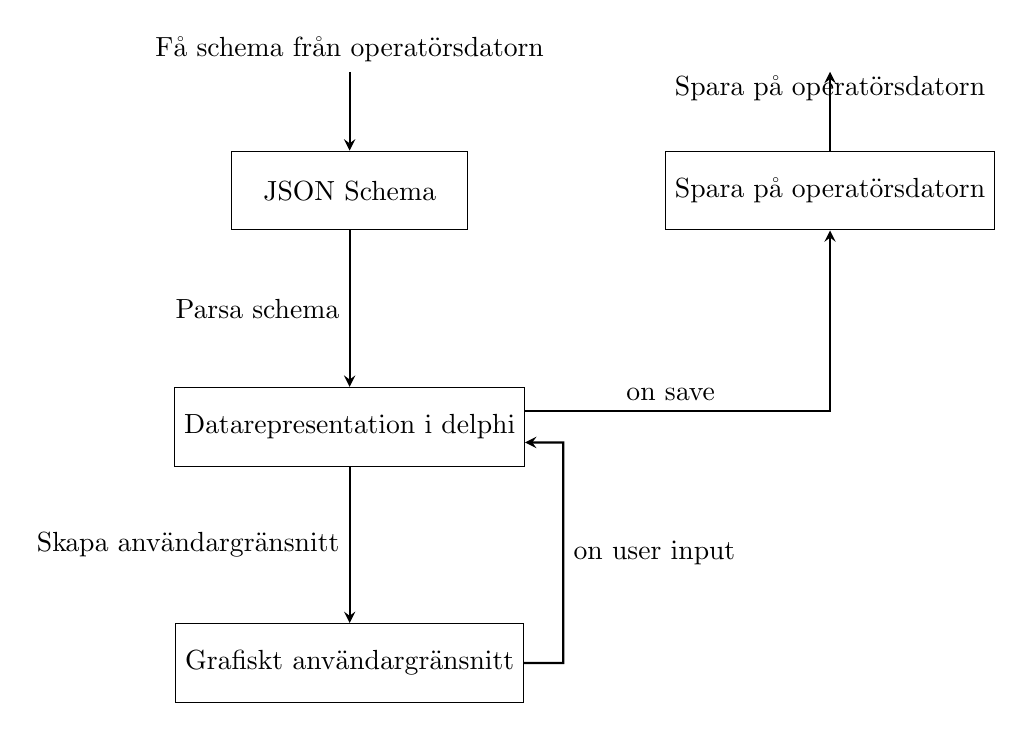
\begin{tikzpicture}
		\node (origin) [defaultnode] {JSON Schema};
		\node (data) [defaultnode, below of=origin, yshift=-2cm] {Datarepresentation i delphi};
		\node (gui) [defaultnode, below of=data, yshift=-2cm] {Grafiskt användargränsnitt};
		\node (save) [defaultnode, right=of origin, xshift=1.5cm] {Spara på operatörsdatorn};
		
		\draw [arrow] (origin) -- node[anchor=east] {Parsa schema} (data);
		\draw [arrow] (data) -- node[anchor=east] {Skapa användargränsnitt} (gui);
		\draw [arrow] (gui.east) -- ++(.5, 0) -- node[anchor=west] {on user input} ++(0, 2.8) -- ([shift={(0, -0.2)}]data.east);
		\draw [arrow] ([shift={(0, 0.2)}]data.east) --  node[anchor=south] {on save} ++ (3.7, 0) -| (save.south);
	
		\draw [arrow] ([shift={(0, 1)}]origin.north) node[anchor=south] {Få schema från operatörsdatorn} -- (origin.north);
		\draw [arrow] (save) -- node[anchor=south] {Spara på operatörsdatorn} ([shift={(0, 1)}]save.north);
	\end{tikzpicture}
\end{figure}

% TODO: Förklara parse

\subsection{Example diagram with TikZ}
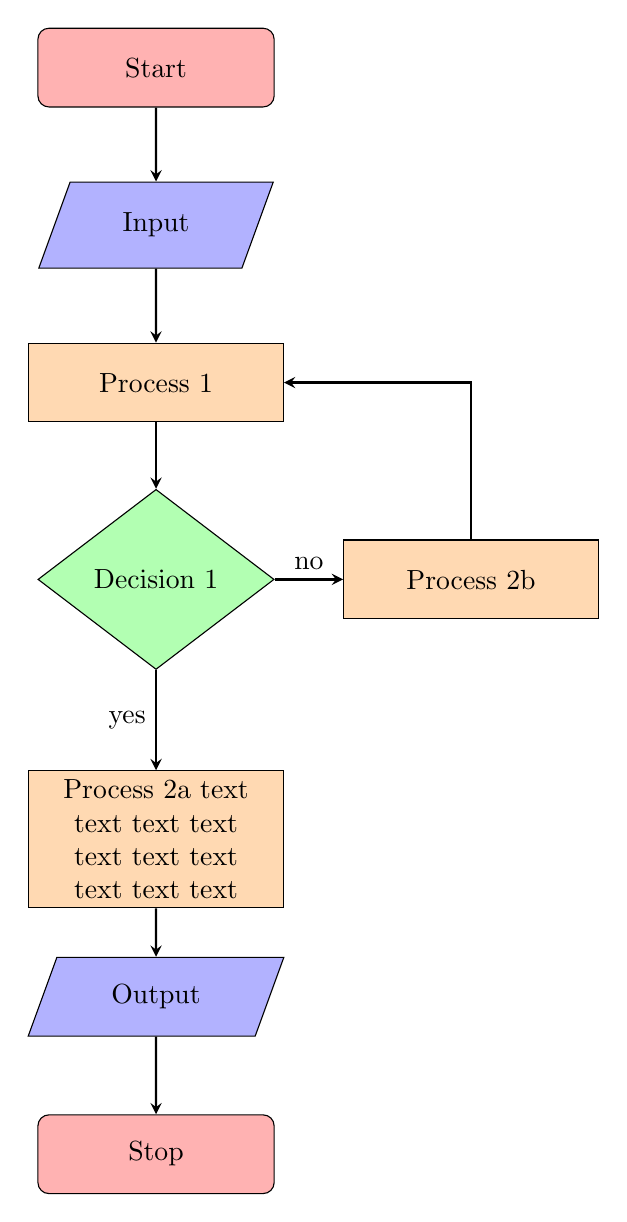
\begin{tikzpicture}[node distance=2cm]
	\node (start) [startstop] {Start};
	\node (in1) [io, below of=start] {Input};
	\node (pro1) [process, below of=in1] {Process 1};
	\node (dec1) [decision, below of=pro1, yshift=-0.5cm] {Decision 1};
	\node (pro2a) [process, below of=dec1, yshift=-1.3cm] {Process 2a text text text text text text text text text text};
	\node (pro2b) [process, right of=dec1, xshift=2cm] {Process 2b};
	\node (out1) [io, below of=pro2a] {Output};
	\node (stop) [startstop, below of=out1] {Stop};
	
	\draw [arrow] (start) -- (in1);
	\draw [arrow] (in1) -- (pro1);
	\draw [arrow] (pro1) -- (dec1);
	\draw [arrow] (dec1) -- node[anchor=east] {yes} (pro2a);
	\draw [arrow] (dec1) -- node[anchor=south] {no} (pro2b);
	\draw [arrow] (pro2b) |- (pro1);
	\draw [arrow] (pro2a) -- (out1);
	\draw [arrow] (out1) -- (stop);
\end{tikzpicture}


\chapter{Resultat}

\section{Vad saknas i JSON Schema}
Hur hanterar man olika valideringsfel?

Föreslå kanske att JSON Schemat som föreslogs i rapport X ska användas.

\section{Hur ska schemat genereras?}

\section{Ett schema för att beskriva schemat}

\section{Datarepresentation i Delphi}
Många språk skiljer på integer och double men det gör varken Javascript, JSON eller JSON Schema


\subsection{JSON Pointer and \$ref}

\section{Användargränsnittet}

\subsection{JSON Editor}
% Vanlig json editor

\subsection{Generaliserat användargränsnitt}
% Nestad form ischhhhhh
	% går ej pga för många inställningar och möjligtvis för djup nestning

\subsection{Användargränsnitt utifrån specifika krav på schemat}
\begin{figure}
	\begin{subfigure}{\textwidth}
		\centering
		\begin{minted}[tabsize=2, frame=lines, fontsize=\small, framesep=2mm]{json}
{
	"$schema": "http://json-schema.org/draft-07/schema",
	"type": "object",
	"properties": {
		"TMimerMainSettings": {
			"title": "Mimer Main Settings",
			"description": "The main settings to set.",
			"type": "object",
			"properties": {
				"MyName": {
					"title": "My Name",
					"description":
						"This is the name that will be shown on a place",
					"type": "string",
					"default": ""
				}
			}
		}
	}
}
		\end{minted}
		\subcaption{Exempel på enkelt JSON Schema}
		\vspace{2em}
	\end{subfigure}
	\begin{subfigure}{\textwidth}
		\centering
		Här ska det finnas en bild med resultatet
		\subcaption{Det resulterande användargränsnittet}
	\end{subfigure}
	\caption{Exempel på enkelt JSON Schema}
\end{figure}

\chapter{Diskussion, slutsats och fortsatt arbete}

\printbibliography[heading=bibintoc] % Print the bibliography (and make it appear in the table of contents)

\appendix

\chapter{Extra Material som Bilaga}

\end{document}
